\chapter{Космические корабли и станции}
\label{ch:spacecraft-space-station}

Глава посвящена исследованию космических кораблей и станций на основе базы знаний международного проекта Викиданные. С помощью SPARQL-скриптов построен список отечественных кораблей и станций, а также временные графики запуска кораблей в нашей стране и в мире, за период с 1960 по 2021 год. Выполнена оценка полноты Викиданных, показавшая, что многие объекты имеют неправильное значение свойства <<частный случай понятия (P31)>>.
\marginnote{\wdProperty{31}{частный случай понятия} = \href{https://www.wikidata.org/wiki/Property:P31}{экземпляр (P31)}}
\section{Экземпляры объекта <<Космические корабли>> и <<Космические станции>>}
Исследуется свойство \wdProperty{31}{частный случай понятия (P31)} и объекты \href{https://www.wikidata.org/wiki/Q25956}{космические станции (Q25956)} и \href{https://www.wikidata.org/wiki/Q40218}{космические корабли (Q40218)}.
Построим список всех космических кораблей с помощью скрипта в листинге~\ref{lst:spaceships}.

\begin{lstlisting}[ language=SPARQL, numbers=none, caption={{\href{https://w.wiki/4By4}{Список кораблей}}\protect\footnotemark}, label=lst:spaceships, ]
# List of spaceсraft (Q40218) and space station (Q25956)
SELECT  ?s ?sLabel ?typeLabel
WHERE
{
  VALUES ?type {wd:Q40218 wd:Q25956}
  ?s wdt:P31 ?type.  # Selecting the type of object
  SERVICE wikibase:label { bd:serviceParam wikibase:language"ru,en"}
}
\end{lstlisting}
\footnotetext{Найдено \num{118} объектов в 2021 году. Ссылка на SPARQL-запрос: \href{https://w.wiki/4By4}{https://w.wiki/4By4}}
\section{Хорошие и плохие объекты}
В 2017 году примерами наиболее полно проработанных экземпляров объекта <<космические станции>> являлись:
\begin{itemize}
  \item\href{https://www.wikidata.org/wiki/Q25271}{МКС};
  \item\href{https://www.wikidata.org/wiki/Q48604}{Мир};
  \item\href{https://www.wikidata.org/wiki/Q131500}{Тяньгун-1}.
\end{itemize}
Примерами плохо заполненных экземпляров объекта <<космические корабли>> в 2017 году были:
\begin{itemize}
  \item\href{https://www.wikidata.org/wiki/Q236448}{Дракон};
  \item\href{https://www.wikidata.org/wiki/Q211727}{Орион};
  \item\href{https://www.wikidata.org/wiki/Q841176}{Восход}.
\end{itemize}
По состоянию на 2021 год наиболее полным и проработанным объектом на Викиданных является \href{ https://www.wikidata.org/wiki/Q184201}{Apollo 8}, имеющий 30 свойств.
Почти пустым и малоинформативным объектами всего с 1 свойством являются: 
\begin{itemize}
  \item\href{https://www.wikidata.org/wiki/Q10491365}{ Europa Astrobiology Lander };
  \item\href{https://www.wikidata.org/wiki/Q6514453 }{ Project Orbiter };
  \item\href{https://www.wikidata.org/wiki/Q5961734 }{ LRK };
  \item\href{https://www.wikidata.org/wiki/Q5327028 }{ EarthForce One };
  \item\href{https://www.wikidata.org/wiki/Q60767924 }{ Soyuz GVK };
  \item\href{https://www.wikidata.org/wiki/Q22907583 }{ CubeSat for Solar Particles }.
\end{itemize}
Для изучения объектов использовался сервис ProWD и соответсвтующий {{запрос}\protect\footnotemark}. Заполнение объктов неравномерное, большая часть заполнены менее, чем на 30%. 
\footnotetext{Запрос для анализа объектов: \href{https://prowd.id/dashboards/79a3b192dfa0/profile}{https://prowd.id/dashboards/79a3b192dfa0/profile}}
\section{Иерархия и вывод космических кораблей}
Была поставлена задача: построить иерархию космических кораблей такую, чтобы в итоговый список космических кораблей включались и транспортные космические корабли, и вымышленные звездолёты, и прочий космический транспорт и на основе этой иерархии написать скрипт, который будет выводить список всех космических кораблей. Космические корабли бывают транспортные (предназначены для людей), грузовые, вымышленные и все остальные. Используем эту иерархию для решения задачи с помощью следующего скрипта~\ref{lst:spaceshipsIE}:

\begin{lstlisting}[ language=SPARQL, numbers=none, caption={{\href{https://w.wiki/4BbU}{Список кораблей различных типов}}\protect\footnotemark}, label=lst:spaceshipsIE, ]
#List of spacecraft 
SELECT  ?spacecraft ?spacecraftLabel   
WHERE
{
  {?spacecraft wdt:P31 wd:Q40218.} UNION #spacecraft
  {?spacecraft wdt:P31 wd:Q18039177.} UNION #fictional spacecraft
  {?spacecraft wdt:P31 wd:Q402330.} #robotic spacecraft
  SERVICE wikibase:label { bd:serviceParam wikibase:language "ru,en"}
}
\end{lstlisting}
\footnotetext{Найдено \num{157} кораблей всех видов в 2017 году. и \num{193} корабля всех видов в 2021 году. Ссылка на SPARQL-запрос: \href{https://w.wiki/4BbU}{https://w.wiki/4BbU}}

\section{Список отечественных кораблей}
Найдем корабли, сконструированные В СССР или России. с помощью скрипта из листинга~\ref{lst:spaceshipsUSSR}:

\begin{lstlisting}[ language=SPARQL, numbers=none, caption={{\href{https://w.wiki/4BbY}{Список отечественных кораблей}}\protect\footnotemark}, label=lst:spaceshipsUSSR, ]
#List of Russian and USSR spacecraft
SELECT  ?spacecraft  ?spacecraftLabel 
WHERE
{
  {?spacecraft wdt:P31 wd:Q40218.} UNION #spacecraft
  {?spacecraft wdt:P31 wd:Q18039177.} UNION #fictional spacecraft
  {?spacecraft wdt:P31 wd:Q402330.}#robotic spacecraft
  {?spacecraft wdt:P17 wd:Q15180. } UNION #USSR
  {?spacecraft wdt:P17 wd:Q159. } #Russia
  SERVICE wikibase:label { bd:serviceParam wikibase:language"ru,en"}
}
\end{lstlisting}
\footnotetext{Найдено \num{3} отечественных корабля в 2017 году. и \num{21}  в 2021 году. Ссылка на SPARQL-запрос: \href{https://w.wiki/4BbY}{https://w.wiki/4BbY}}

\section{Анализ полноты Викиданных}
До полноты Викиданным в области космических кораблей и станций крайне далеко. Если по запросу обо всех кораблях вывелось 193 результата, то по запросу об отечественных кораблях всего 21. Это говорит о том, что данные не полны. В статьях русской Википедии \href{https://ru.wikipedia.org/wiki/%D0%9A%D0%BE%D1%81%D0%BC%D0%B8%D1%87%D0%B5%D1%81%D0%BA%D0%B0%D1%8F_%D0%BF%D1%80%D0%BE%D0%B3%D1%80%D0%B0%D0%BC%D0%BC%D0%B0_%D0%A1%D0%A1%D0%A1%D0%A0}{Космическая программа СССР} и \href{https://ru.wikipedia.org/wiki/%D0%9A%D0%BE%D1%81%D0%BC%D0%BE%D0%BD%D0%B0%D0%B2%D1%82%D0%B8%D0%BA%D0%B0_%D0%A0%D0%BE%D1%81%D1%81%D0%B8%D0%B8}{Космонавтика России} можно насчитать как минимум 45 космических кораблей, спроектированных в СССР и России. То есть в викиданных представлено менее половины от всех отечественных кораблей, однако ситуация стала значительно лучше по сравнению с 2017 годом, когда по запросу к викиданным выдавалось менее 10% от всех кораблей. 

\section{Временные графики освоения космоса в нашей стране и мире}
Скрипт построения графика запуска космических аппаратов в нашей стране, начиная с 1960-х годов, представлен в листинге~\ref{lst:imageRU}.
\begin{lstlisting}[ language=SPARQL, caption={{\href{https://w.wiki/4QGX}{Запуски в СССР и России}}\protect\footnotemark}, label=lst:imageRU, ]
# The number of spacecraft launches in Russia every 5 years
#defaultView:BarChart
SELECT (STR(?lapse) AS ?lapse_str) (COUNT(?item) AS ?quantity)
WHERE {                  # spacecraft belongs to
        {?item wdt:P17 wd:Q15180} # Soviet Union
  UNION {?item wdt:P17 wd:Q159}.  # or Russia
  
  ?item wdt:P619 ?launch. # date of spacecraft launch (P619)
  BIND( YEAR(?launch) AS ?year) 
  BIND(FLOOR(?year/5)*5 AS ?lapse) # count for each 5 years
SERVICE wikibase:label {bd:serviceParam wikibase:language "ru,en"}
} 
GROUP BY ?lapse
ORDER BY ?lapse # Order 1970, 1975, 1980, ...
\end{lstlisting}
\footnotetext{Найдено \num{14} результата в 2021 г. Ссылка на SPARQL-запрос: \href{https://w.wiki/4QGX}{https://w.wiki/4QGX}}
Свойство Р619 (дата запуска космического корабля) позволяет получать количество запусков кораблей в указанный период, что в рамках данного скрипта заменяет набор свойств Р31 (частный случай понятия), так как фильтрация по запускам кораблей позволяет отказаться от дополнительных фильтров для проверки корабля. В случае отсутствия функции STR в 3 строке год запуска (lapse) рассматривается как число, что приводит столбчатую диаграмму к виду графика, где горизонтальная ось отвечает за год запуска, а результаты обозначаются точками с координатами (год, запуски). UNION позволяет объединить запуски России и СССР. В строке 10 производится подсчёт количества за пятилетку, от года Х до Х+5. В строке 13 результаты группируются по пятилеткам. Переменная lapse отвечает за накопление данных за период, переменная quantity указывает, что в рамках скрипта требуется воспринимать объекты как их количество.

\begin{figure*}[h!]
  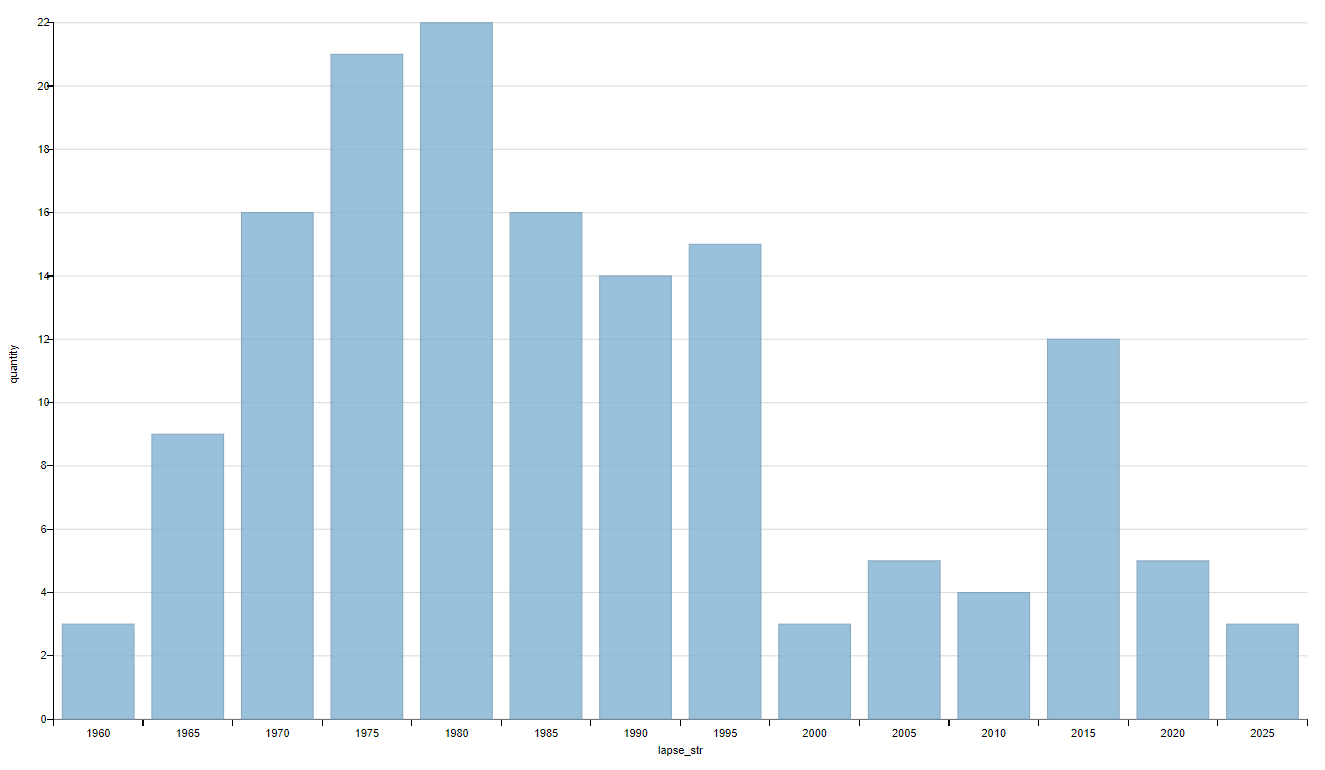
\includegraphics[width=\linewidth]{graphics/chapter/spacecraft_space_station/ImgRU.png}
  \caption[График Россия]{Визуализация количества запусков космических кораблей а России каждые 5 лет 2021 SPARQL}%
  \label{fig:ImageRU5}%
\end{figure*}

Из графика ~\ref{fig:ImageRU5} можно увидеть, что самый активный период развития космонавтики в нашей стране был в 1970-1995 годах.
Скрипт построения графика запусков космический кораблей в мире по годам и странам представлен в листинге ~\ref{lst:imageALL}:
\begin{lstlisting}[ language=SPARQL, numbers=none, caption={{\href{https://w.wiki/4bEu}{Запуски в мире}}\protect\footnotemark}, label=lst:imageALL, ]
# Diagram of spacecraft launches by year and country
#defaultView:BarChart
SELECT ?year (COUNT(?obj) AS ?count) ?country ?countryLabel
WHERE {
  ?obj wdt:P17 ?country. # spacecraft belongs to country 
  ?obj wdt:P619 ?launch. # date of spacecraft launch
  BIND(str(YEAR(?launch)) AS ?year)
  
  SERVICE wikibase:label {bd:serviceParam wikibase:language "ru".}
}
GROUP BY ?year ?country ?countryLabel
\end{lstlisting}
\footnotetext{Найдено \num{328} результата в 2021 г. Ссылка на SPARQL-запрос: \href{https://w.wiki/4bEu}{https://w.wiki/4bEu}}

\begin{figure*}[h!]
  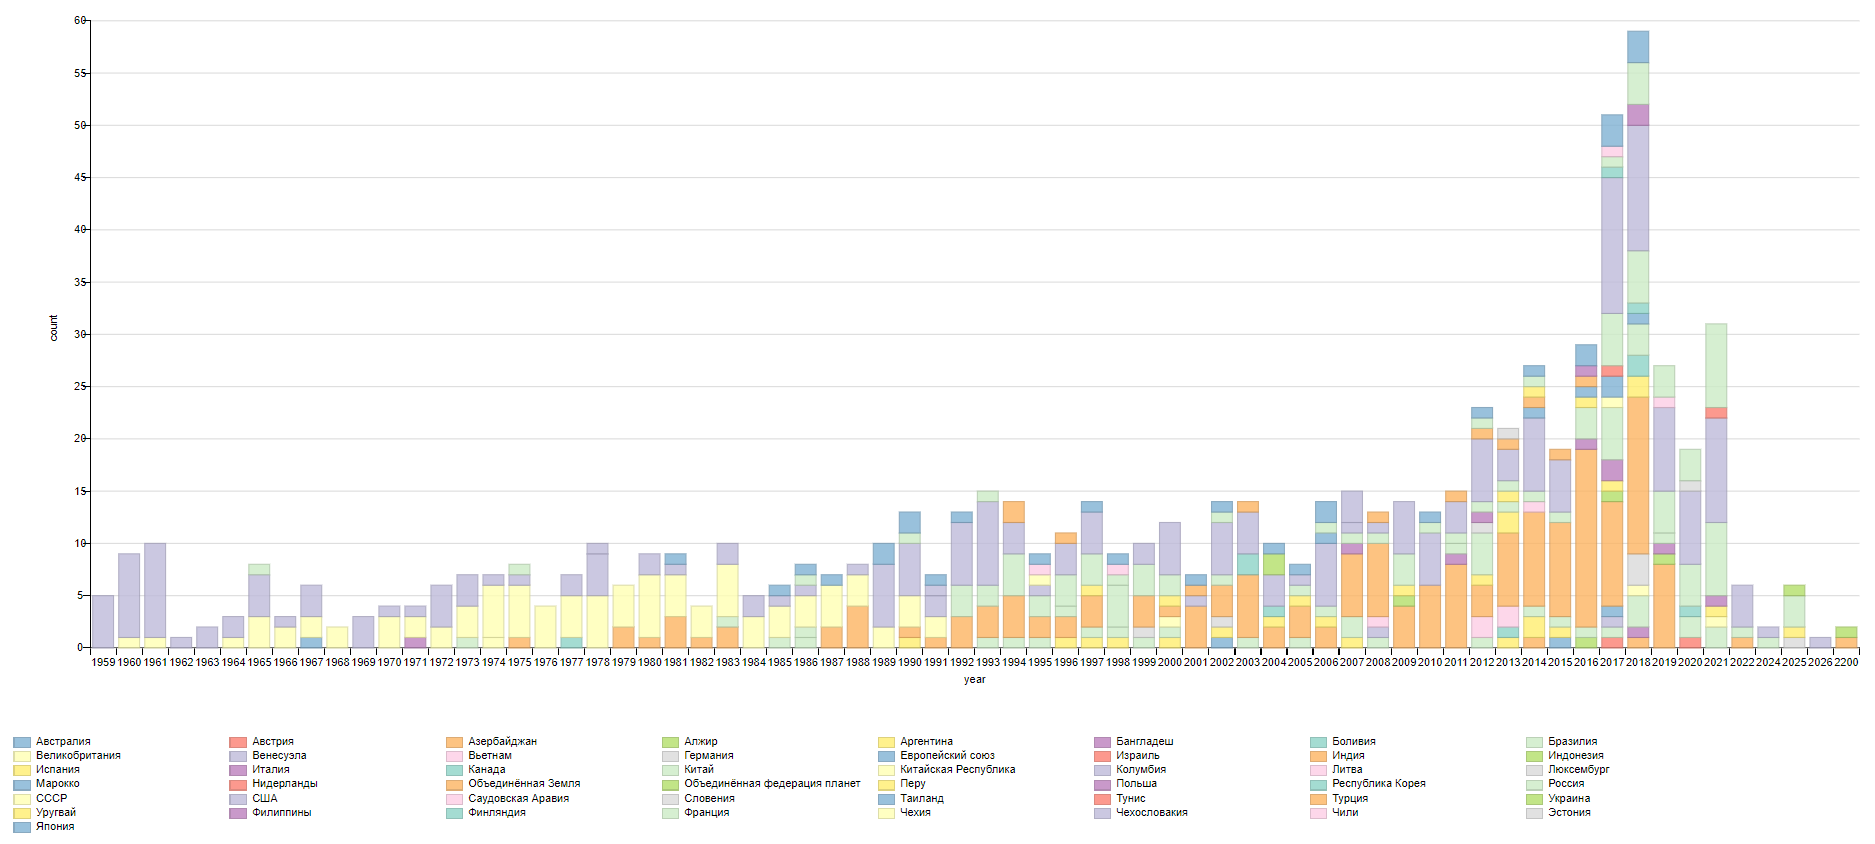
\includegraphics[width=\linewidth]{graphics/chapter/spacecraft_space_station/Visualization of the number of spacecraft launches by year and country 2021.png}
  \caption[График мир]{Визуализация количества запусков космических кораблей по годам и странам 2021 SPARQL}%
  \label{fig:ImgALL}%
\end{figure*}

Из графика ~\ref{fig:ImgALL} можно увидеть, что по состоянию на 2021 год в Викиданных превалируют данные о запусках США и Индии (только у них зафиксировано более 10 графков в год). Пик запусков был в 2018 году (59 штук). По информации из Викиданных российская космонавтика занимает средние позиции по количеству запусков, её численные показатели за последние 5 лет схожи с показателями СССР 1975-1980 годов и составляют около 5 запусков в год.

\section{Будущая работа}
\begin{itemize}
  \item Подсчитать и вывести список кораблей, которые отправились или планируется отправить на Марс.
  \item Подсчитать и построить график доли кораблей, предназначенных для отправки на Марс, по отношению к кораблям отправленным на Луну.
  \item Найти корабли, которые не смогли выйти на орбиту.
\end{itemize}
